% !TeX root = ../main.tex
% Add the above to each chapter to make compiling the PDF easier in some editors.

\chapter{Awareness}

This chapter is going to introduce \gls{wa}, as a tool for developing productive collaboration systems. We will start by looking at the \gls{sa}, as it serves as the theoretical foundation that the concept of \gls{wa} builds upon.

% TODO: give examples of using auditory cues in situation (maybe, some of endsley papers) and workspace awareness (gutwin 2002, ?Ammi, Katz, "Intermodal audio–haptic intermodal display..")
% meh - TODO: human factors? I mention the control mapping or correspondense building a couple of times.
% TODO: 



\section{Situation Awareness}
% This section serves as a pre-cursor to the Workspace Awareness section, and shows the base that WA is built upon.

%Situation awareness itself
\gls{sa} is usually used in attention-critical and hazardous tasks, where failure to react to the a change in a system might cause serious and even lethal consequences. SA served as one of the base notions, on which the concept of the workspace awareness was built.

\gls{sa} has seen great development through its application in the aviation field, and \cite{endsley_situation_1988} defines it as a combination of: perception of the elements in the certain volume around the user at the given time; comprehension of the meaning of these elements; and the ability to project their state into the nearest future.

[Not finished. TODO: More info from \cite{endsley_situation_1988} (human factors, levels of awareness, etc.)]
%* Write about the jet fighter simulator somewhere
%o Human factors?
%o Levels of awareness // <- I will classify my system according to this in the end

\paragraph{Measurement}
\cite[p.~791-792]{endsley_situation_1988} reviews different approaches to the measurement of \gls{sa} that help system designers answer the fundamental question: "Does system A promote better SA than system B?". In the author's opinion, all the approaches that were available up to that point suffer from their own individual limitations. For example, the subjective approach, where the subject is asked to rate his \gls{sa} from 1 to 10 suffers from 2 major drawbacks: first, the subject is not aware of "what is really going on in the environment", and secondly, the outcome of the task can influence the rating. Similarly, the psychological approach suffers from the incomplete human-computer interfaces to monitor what is going on with the pilot at this moment, and what they are thinking about. Finally, if the questionnaires are used, the fact that humans are not that good at recalling past mental events comes into play. Another set of problems arises, if an attempt is made to solve the issue with the questionnaire approach by querying pilots in real-time, such as the pilots can start to attend to the information they are questioned upon more thoroughly or they can be under a heavy load at the moment of questioning, which would obstruct their answer.

Nevertheless, \cite{endsley_situation_1988} finds the biggest limitation of the mentioned approaches was that they attempted to evaluate only a single design issue at the time. All this leads \cite{endsley_situation_1988} to introduce the \gls{sagat}. The idea here is that, first, the task goes though goal-directed analysis to determine the \gls{sa} requirements: the goal, subgoals, decisions required to actualize the given subgoal, and the knowledge required on all three levels of \gls{sa} (\ref{fig:sagoalorientedtaskanalysis}). 
\begin{figure}
	\centering
	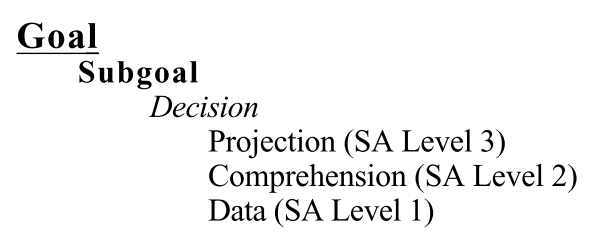
\includegraphics[width=0.7\linewidth]{figures/placeholders/SA_goal_oriented_task_analysis}
	\caption{Format of Goal-Directed Task Analysis (totaly spizgenoe name from: \cite{endsley_direct_nodate})}
	\label{fig:sagoalorientedtaskanalysis}
\end{figure}
This should yield an extensive list of questions, which assess SA information the \gls{sa} information of primary and secondary importance (for an example of the results of such analysis, see the Fig. \ref{fig:sagoalorientedtaskanalysisresultexample}).
\begin{figure}
	\centering
	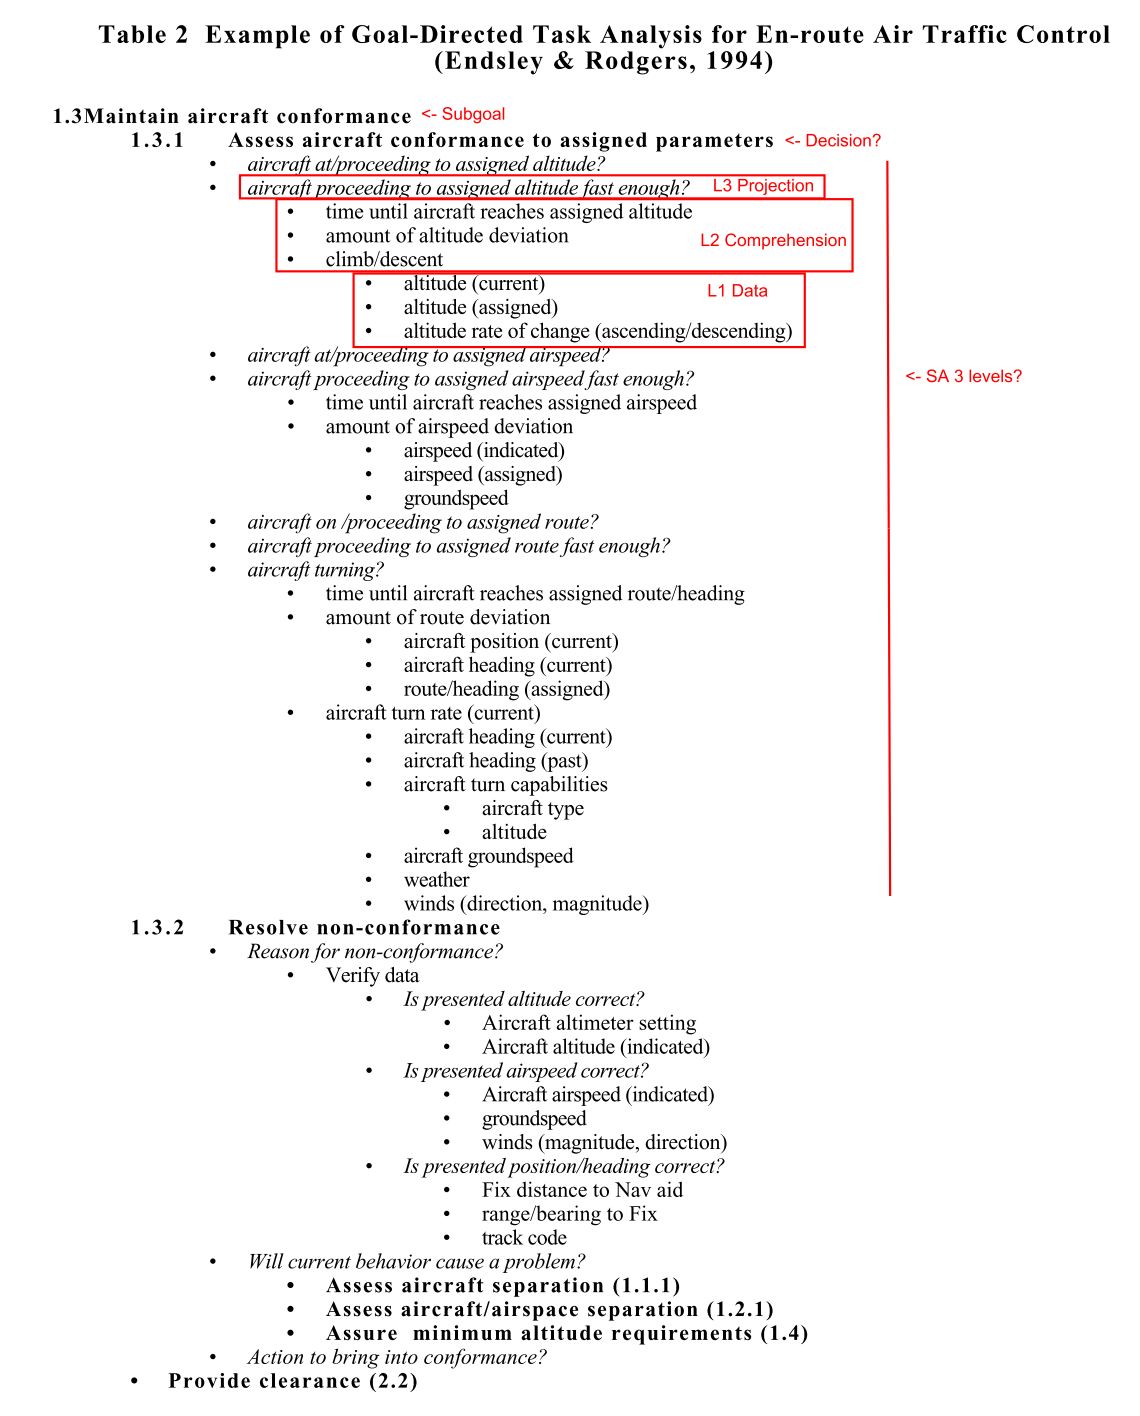
\includegraphics[width=0.7\linewidth]{figures/placeholders/SA_goal_oriented_task_analysis_result_example}
	\caption{Example of Goal-Directed Task Analysis for En-route Air Traffic Control (Endsley \& Rodgers, 1994) [from: \cite{endsley_direct_nodate}]}
	\label{fig:sagoalorientedtaskanalysisresultexample}
\end{figure}
Next, at some point in time, the simulation is halted, and the pilots are queried on the randomly selected questions from the list. When the simulation halts, all the control panels, the ?windshield of the jet-fighter, and other simulation elements are grayed-out. Not every pilot is queried on every question, the goal is to reach the desired statistical significance of the results by assessing a certain number of participants.

% This paragraph is a bit repetetive
By using this approach, it is possible to get a snapshot of the current situation in the point of view of the pilot, which is unbiased by the recall difficulties, and that can be compared to the actual situation after the experiment. Additionally, pilots' \gls{sa} is not artificially enhanced, because the questions do not always directly address the main goals in the current situation, but can concern secondary information, which is still relevant.

\cite{endsley_direct_nodate} notes that, since the introduction of \gls{sagat}, there is practical evidence that the method is valid, reliable, non-intrusive (in case of the halts are made at unpredictable time points), and is able to properly "reliably tap into memory stores" acting as a \gls{sa} index. 


o Bridge to Workspace Awareness


\section{Workspace Awareness}
% Definition
\gls{wa} can be described as "the up-to-the-moment understanding of another person’s interaction with the shared workspace" \cite{gutwin_descriptive_2002}. While this is a trivial task in real-world face-to-face collaboration, \gls{wa} becomes a bottleneck for productive collaboration because of limited information that systems usually provide, and unfamiliar interaction interfaces.
 
% Description
It is an extension of the concept of \gls{sa}, research from the \gls{hci} and \gls{cscw} fields, and authors' own observations and research. \gls{wa} could be characterized as an adaptation of \gls{sa} to the day-to-day working scenarios. This was desired, because as authors put it: "sorting slides on a table does not seem very similar to air combat in a jet fighter" \cite{gutwin_descriptive_2002}, or in our case, to architectural collaboration in immersive \gls{vr} environment. Another major difference of \gls{sa} and \gls{wa} is that besides maintaining their \gls{sa} and performing the domain (their personal) task, collaborators have to perform their collaboration.

% Framework 'classification'
This led \cite{gutwin_descriptive_2002} to develop the \gls{wa} framework, which concerns itself with providing a toolset for describing and analyzing medium-sized workspaces. The framework is applicable to real-time distributed groupware for shared environments, and small mixed-focus collaboration groups busy with generation and execution tasks.
% Framework descriprion
The \gls{wa} framework is split in 3 parts: "What information makes up \gls{wa}?", "How is \gls{wa} information gathered?", "How is \gls{wa} used in collaboration?". 
In Part I the authors address the information that collaborators might require from the workspace. While this can be any type of information, it can be categorized into the most common types. For example, the category "Who" concerns itself with the presence, identity, and authorship questions, and contains the following questions: "Is anyone else in the workspace?", "Who is participating? Who is that?", and "Who is doing that?". An example for the "Who" category can be seen in Fig. \ref{fig:watechniquesforwhoquestions}. There are 8 categories of questions in Part I of the framework: questions about the present (Who?, What?, Where?), and questions about the past (How?, When?, Who? (past), Where? (past), What? (past)). The \gls{wa} framework doesn't concern itself with the information about the future, because this requires projection.
This part of the framework allows designers to compare and design awareness support in different groupware applications by providing a fixed vocabulary for describing their systems.

Part II of the framework deals with the ways the information can be delivered to the users. The authors present 3 ways in which the information can be communicated in a workspace: through bodies and consequential communication, through artifacts and feedthrough, and through conversation, gesture, and intentional communication. While the last one speaks for itself, the first two deal with information transfer through the consequence of people's actions in the workspace, and the information emitted by the manipulated objects in the workspace (for example, a characteristic sound initiated by a person drawing in the workspace).
By considering the different ways in which the information transfer can occur, system designers can make an educated decision about what approach to use in a particular situation.

Part III of the framework turns to the question of how we make use of the information we gather through \gls{wa}. Here we discover 5 types of activities that benefit our \gls{wa} in some way: management of coupling, simplification of communication, coordination of actions, anticipation, and assistance (see summary in Fig. \ref{fig:summaryofactivitieswherwacanbeused}).
This part of the framework allows awareness designers consider different ways people make use of the awareness information, and decide where, whether, and how much of this information is required.
For example, if we take anticipation, "People anticipate others in several ways. They can prepare for their next action in a concerted activity, they can avoid conflicts, or they can provide materials, resources, or tools before they are needed".


\begin{figure}
	\centering
	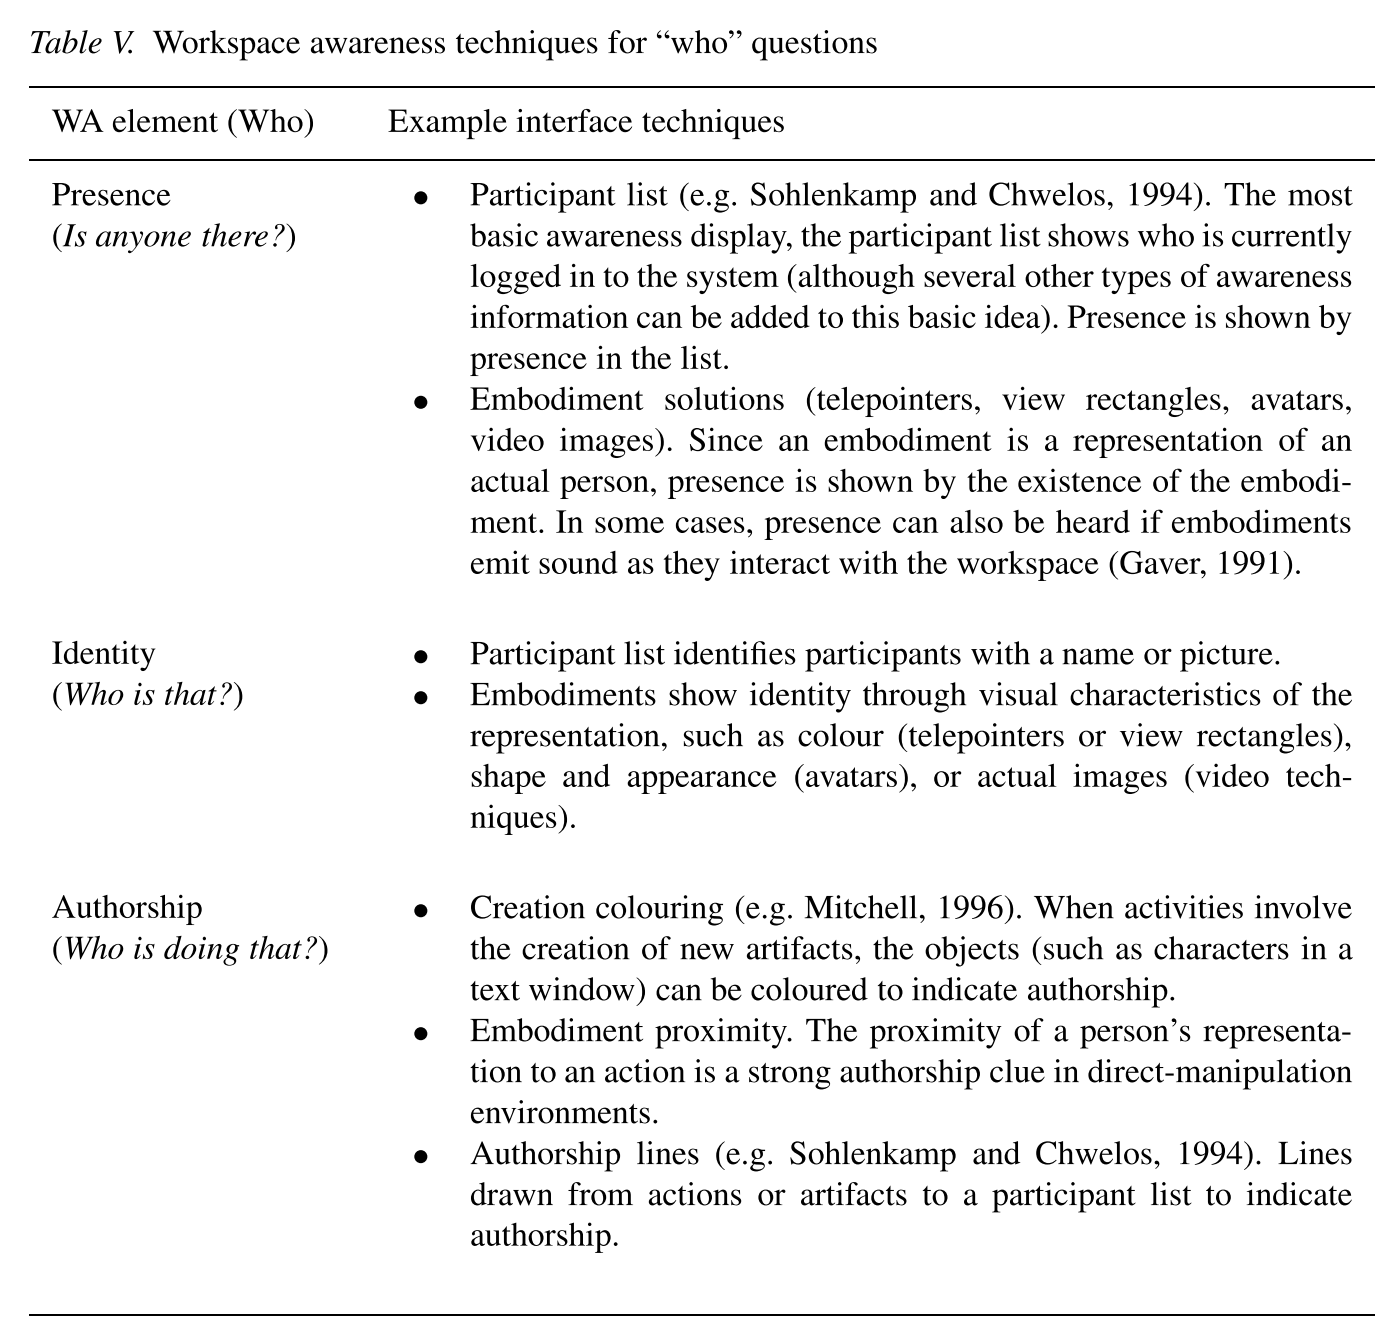
\includegraphics[width=0.7\linewidth]{figures/placeholders/WA_techniques_for_WHO_questions}
	\caption{}
	\label{fig:watechniquesforwhoquestions}
\end{figure}

\begin{figure}
	\centering
	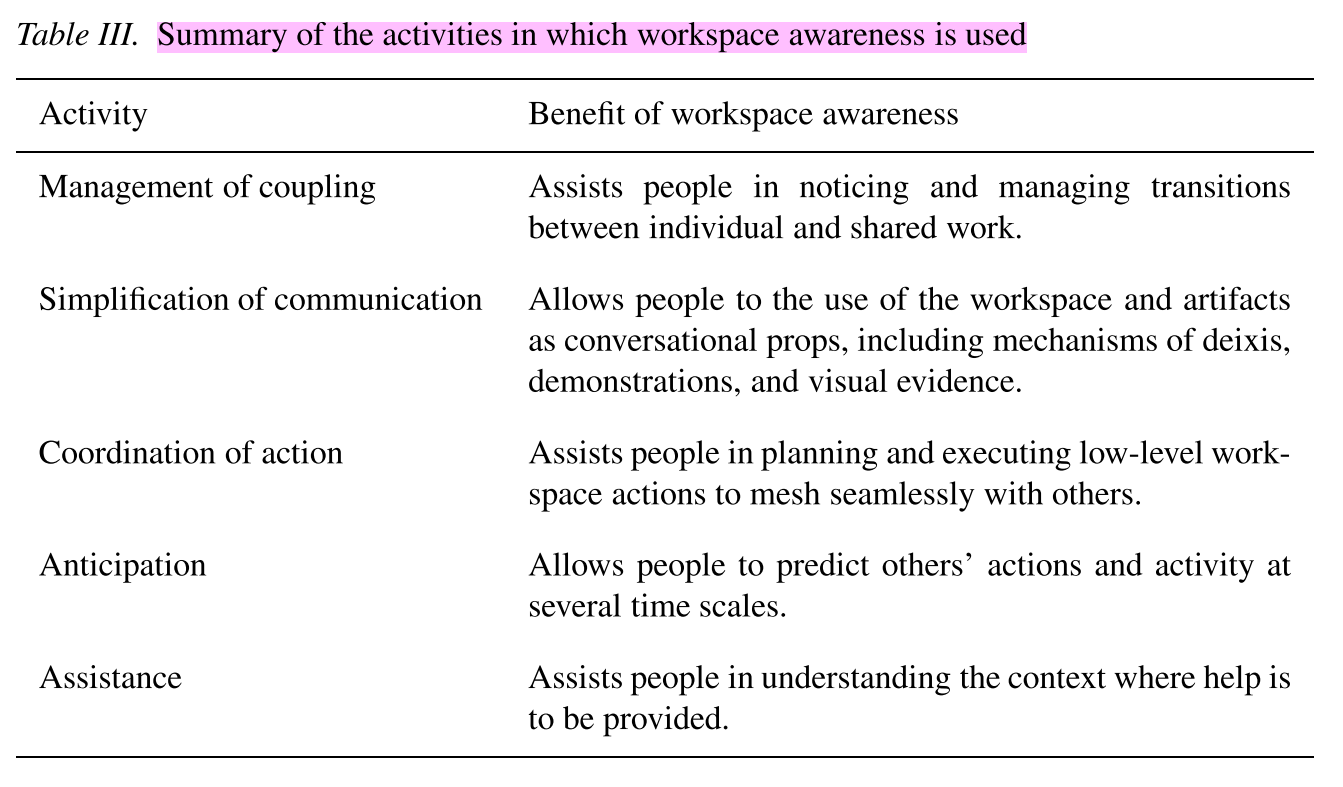
\includegraphics[width=0.7\linewidth]{figures/placeholders/summary_of_activities_wher_WA_can_be_used}
	\caption{}
	\label{fig:summaryofactivitieswherwacanbeused}
\end{figure}


The figure summarizing the framework:

\begin{figure}
	\centering
	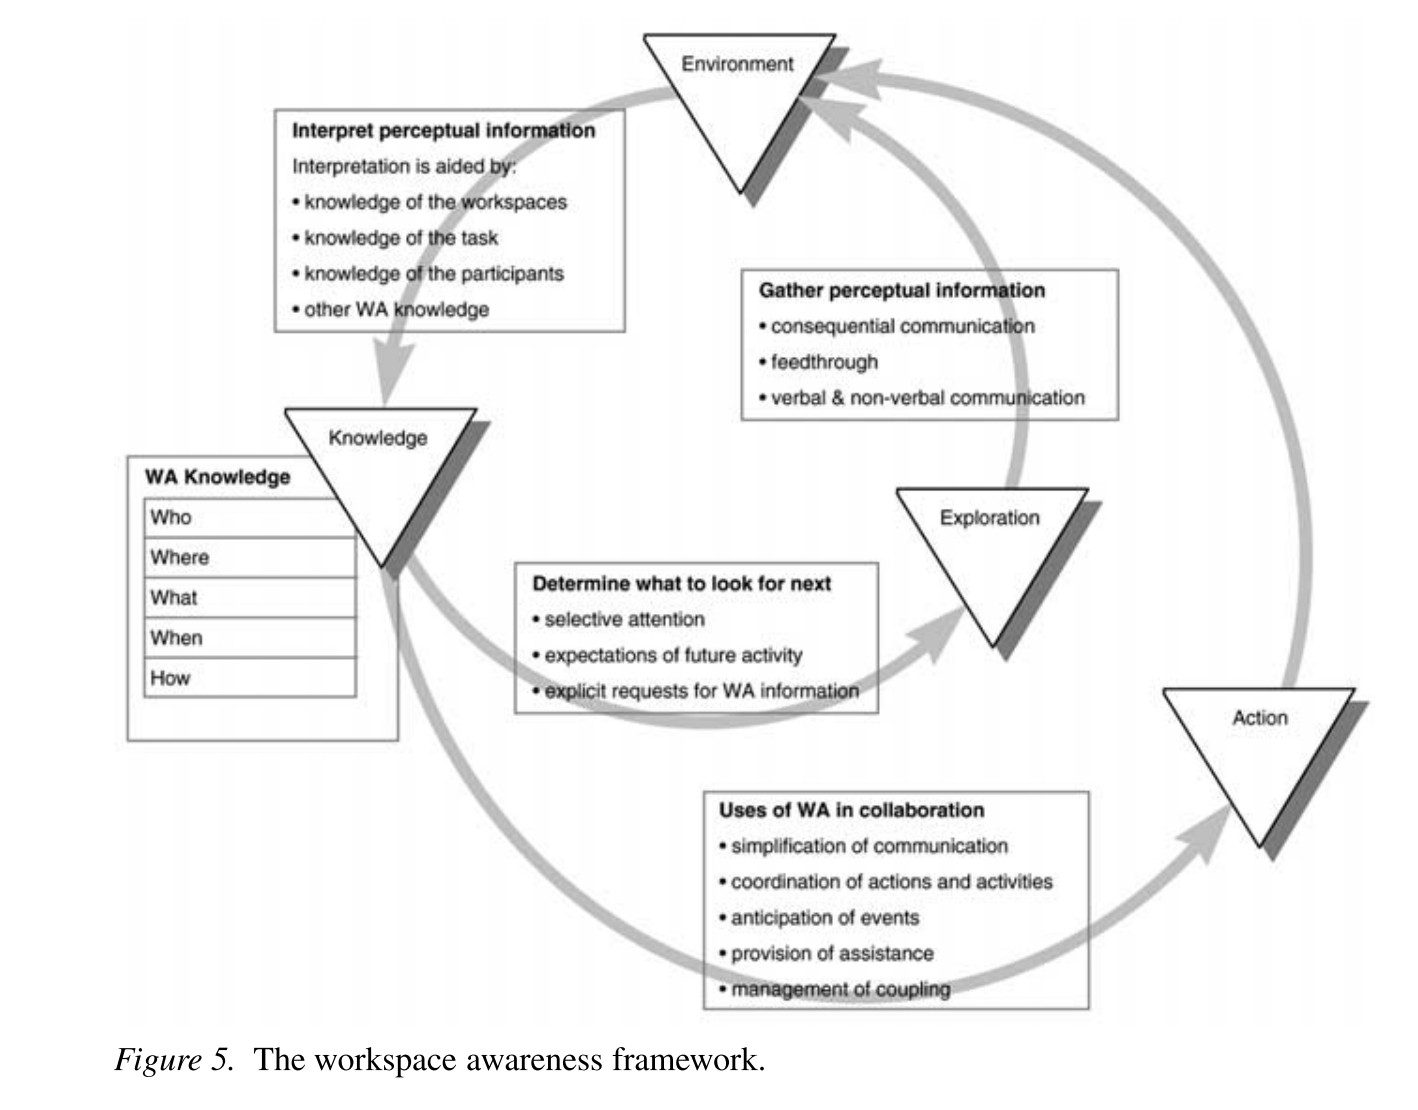
\includegraphics[width=0.7\linewidth]{figures/placeholders/WA_framework}
	\caption{}
	\label{fig:waframework}
\end{figure}


%o Relation to human factors’ research?

* Measurement
?SAGAT is sorta not applicable, because not so many elements to query upon.
o Bridge to Sonification: 
* Awareness - secondary/monitoring task \& sonification is great for monitoring -> use it for our experiment 
"Awareness is a secondary goal in the task – that is, the overall goal is not simply to maintain awareness but to complete some task in the environment"

